\chapter{Codifica di Sorgente}

Ci inoltriamo finalmente nel cuore della teoria dell'informazione, ovvero la codifica di sorgente.

\section{Sorgenti e Codifica}

\begin{definition}{Sorgente (discreta e a memoria zero)}
  Chiamiamo \keyword{Sorgente discreta e a memoria zero} una variabile aleatoria discreta, identificabile come una coppia \(S = (\SCal,p)\), con \(\SCal\) alfabeto finito, e \(p\) distribuzione su \(\SCal\).
\end{definition}
$\SCal$ viene spesso detto \textit{alfabeto sorgente}. Inoltre, se \(p\) è una distribuzione positiva, \(S\) viene detta \textbf{sorgente propria}.

\begin{definition}{Codifica}
  Definiamo \keyword{codifica} un morfismo iniettivo \(\varphi: \SCal^* \to A^*\) con \(A\) alfabeto. Il morfismo $\varphi$ identifica il \keyword{codice} $X=\varphi(\SCal)$.
  Diremo inoltre che $X$ è \keyword{adattabile} alla sorgente \(S\) se \(\# X = \# \SCal\).
  In particolare, $X$ sarà \keyword{adattato} a una sorgente \(S\) mediante una biiezione \(\varphi_{|_X}: \SCal \leftrightarrow X\).
\end{definition}
Se $X$ è adattabile, allora, per ottenere la biiezione che lo adatta alla sorgente, è necessario forzare la suriettività di $\varphi$, definita iniettiva, restringendo $\varphi$ a $\varphi^{-1}(X)$.

\begin{definition}{Costo di una codifica}
  Data una sorgente \(S = (\SCal,p)\) e una codifica \(\varphi: \SCal^* \to A^*\) con codice \(X = \varphi(\SCal)\), definiamo il \keyword{costo} di \(\varphi\) la quantità:
  \[c(X,\varphi) = \sum_{s \in \SCal} p(s) \abs{\varphi(s)}\]
  ovvero la media pesata sulla distribuzione \(p\) delle lunghezze delle parole codificate.\\
  Il \keyword{costo assoluto} di un codice \(X\) sarà
  \[c(X) = \min_{\varphi: \varphi(\SCal) \leftrightarrow  X} c(X,\varphi)\] ovvero il costo associato alla codifica che per cui si ottiene il costo minimo.
\end{definition}

\begin{example}[label=ex:codifica]{}
  Sia \(\SCal = \set{s_1,s_2,s_3}\), \(A = \set{a,b}\), \(X = \set{a,ba,bb}\).
  Se \(p(s_1) = 1/2, p(s_2) = p(s_3) = 1/4\), e inoltre \(\varphi(s_1) = ba, \varphi(s_2) = a, \varphi(s_3) = bb\), si ha che
    \[c(X,\varphi) = \frac{7}{4} > c(X) = \frac{3}{2}\]
  dove $c(X)$ è il costo ottenuto scegliendo la codifica $\varphi'$ che associa probabilità maggiori a parole di $X$ più corte, ovvero associa la probabilità massima alla parola più corta, la seconda probabilità massima alla seconda parola più corta e così via. 
\end{example}

La scelta di $\varphi'$ nell'esempio non è casuale, ma è anzi il risultato della seguente proposizione.

\begin{proposition}{}
  Sia \(S\) sorgente, \(X\) codice su \(A\) \emph{adattato} a \(S\) mediante \(\varphi\).
  Allora \(c(X) = c(X,\varphi)\) se e solo se
    \[\forall s,s' \in \SCal, p(s) < p(s') \implies \abs{\varphi(s)} > \abs{\varphi(s')} \]
\end{proposition}

\begin{definition}{Codice ottimale}
  Diremo che \(X\) è un \keyword{codice ottimale} per la sorgente \(S\) se, per ogni codice \(Z\) sullo stesso alfabeto e di cardinalità \(\#X=\#\SCal\), si ha che
  \[c(X) \leq c(Z)\]
\end{definition}

In altre parole, un codice è ottimale se il suo costo assoluto è minore o uguale di qualsiasi altro costo assoluto ottenuto a partire da un altro codice sullo stesso alfabeto e con stessa cardinalità.

\begin{example}{}
  Data la sorgente dell'esempio~\ref{ex:codifica}, il codice \(Z = \set{aa,ba,bb}\) \textbf{non} è ottimale, poiché \(c(Z) = 2\), mentre abbiamo trovato un codice di costo inferiore nell'esempio precedente.
\end{example}

\section{Entropia di una sorgente}

\begin{definition}{Entropia di una sorgente}
  Data una sorgente \(S = (\SCal,p)\), definiamo l'\keyword{entropia} di \(S\) la quantità
  \[H(S) = -\sum_{s \in \SCal} p(s) \log\left(p(s)\right) = \sum_{s \in \SCal} p(s) \log\left(\frac{1}{p(s)}\right)\]  
\end{definition}

Tale quantità rappresenta un valore medio dell'autoinformazione (ovvero dell'incertezza) della sorgente.
La base del logaritmo non è specificata in quanto cambierebbe il valore di $H(S)$ solo di una costante moltiplicativa dovuta al cambio di base. Tale costante moltiplicativa è del tutto analoga ad un cambio di unità di misura.

Infatti, l'entropia (e l'informazione in generale) si misura utilizzando comunemente tre unità di misura:
\begin{itemize}
  \item \emph{hartley} (base \(10\)), prima unità di misura dell'informazione;
  \item \emph{nat} (base \(e\)), utile per alcune formulazioni matematiche;
  \item \emph{bit} (base \(2\)), più utilizzata al giorno d'oggi.
\end{itemize}
L'entropia di \(1 bit\) è quella di una sorgente binaria uniforme:
\[H(S) = \frac{1}{2}\log_2(2) + \frac{1}{2}\log_2(2) = 1\]
Da questo momento in avanti si farà riferimento unicamente ai \(bit\) come unità di misura dell'informazione, omettendo dunque la base del logaritmo e assumendola pari a $2$.

\begin{note}[label=note:entropy-continuity-assumption]{}
  La definizione di entropia fornita non esclude la possibilità di avere \(p(s) = 0\) per qualche \(s \in \SCal\).
  In tal caso il termine della somma corrispondente a tale \(s\) non sarebbe definito, in quanto si otterrebbe una forma indeterminata $0\cdot -\infty$.
  Dunque, per fornire continuità a $H$, si assume \(p(s)\log\left(p(s)\right) = 0\), dato che è noto che \(\lim_{x \to 0^+} x \log\left(x\right) = 0\).

  In maniera formale, si può ridefinire l'entropia come
  \[H(S) = -\sum_{s \in \SCal} h(s)\]
  dove
  \[h(s) = \begin{cases}
              p(s) \log\left(p(s)\right) & , p(s) > 0 \\
              0 & , p(s) = 0
            \end{cases}
  \]
\end{note}

Andiamo adesso a dimostrare che l'entropia è sempre dotata di un limite inferiore e di un limite superiore.

\begin{proposition}[label=prop:lower_bound_entropy]{Limite inferiore dell'entropia}
  Sia $S=(\mathcal{S},p)$ una sorgente discreta a memoria zero. Allora si ha $H(S)\geq 0$.\\
  Inoltre, $H(S)=0 \iff \exists !\bar{s}\in \mathcal{S}:p(s)=1$.
\end{proposition}

\begin{proof}
  Poiché \(\forall s \in \SCal: 0\leq p(s) \leq 1\), abbiamo che\footnote{È denotato che \(-\infty \leq \log\left(p(s)\right)\) e non \(-\infty < \log\left(p(s)\right)\), poiché si assume \(\log\left(0\right)\) definito come \(-\infty\) per continuità.}
  \[-\infty \leq \log\left(p(s)\right) \leq 0 \iff  0 \leq -\log\left(p(s)\right) = \log\left(\frac{1}{p(s)}\right) \leq \infty\]

  Dunque \(H(S) = \sum_{s \in \SCal} p(s) \log\left(\frac{1}{p(s)}\right) = \mathbb{E}[\log\left(\frac{1}{p(S)}\right)] \geq 0\), essendo somma pesata di quantità non negative.

  Inoltre, se \(p(s) = 1\) e \(p(t) = 0, \forall t \in \SCal \setminus \set{s}\) si ha che
  \[H(S) = 1 \cdot \log\left(\frac{1}{1}\right) - \sum_{t \in \SCal \setminus \set{s}} 0 \cdot \log\left(0\right) = 0 - 0 = 0\]
  Viceversa, se \(H(S) = 0\), deve aversi \(p(s) \log\left(\frac{1}{p(s)}\right) = 0, \forall s \in \SCal\), che può avvenire solo in due casi, ovvero \(\forall s \in \SCal (p(s) = 0 \lor p(s) = 1)\).
  Poiché \(p\) è una distribuzione di probabilità, si ha \(\sum_{s \in \SCal} p(s) = 1\), e dunque
  \[\exists!\bar{s} \in \SCal: p(\bar{s}) = 1\]
\end{proof}

\begin{proposition}[label=prop:upper_bound_entropy]{Limite superiore dell'entropia}
  Sia $S=(\mathcal{S},p)$ una sorgente discreta a memoria zero e $k=\#\mathcal{S}$. Allora si ha $H(S)\leq \log k$.\\
  Inoltre, $H(S)=\log k \iff \forall s \in \mathcal{S}:p(s)=\frac{1}{k}$.
\end{proposition}

Per dimostrare questa proposizione, abbiamo bisogno di un risultato di Analisi matematica: la disuguaglianza di Gibbs.

Siano $p,q$ distribuzioni su $\mathcal{S}$. Allora:
\begin{equation}\label{eq:gibbs}
H(S)=\sum_{s \in \mathcal{S}}{p(s)\log\left( \frac{1}{p(s)} \right)} \leq \sum_{s \in \mathcal{S}}{p(s)\log\left( \frac{1}{q(s)} \right)}
\end{equation}
e vale con il segno uguale solo se $p=q$.

\begin{note}{}
  Si noti che la somma a destra può divergere, poiché non vale l'assunzione \ref{note:entropy-continuity-assumption} in quanto i due termini della somma appartengono a due distribuzioni distinte. Infatti, potrebbe esistere un $s \in \mathcal{S}: p(s) \neq 0 \wedge q(s)=0$ per cui si avrebbe $p(s)\log\left( \frac{1}{q(s)} \right)=\infty$.\\
  Affinché la somma a destra non diverga, è sufficiente imporre che $p$ e $q$ siano distribuzioni positive.
\end{note}

\begin{proof}[Dimostrazione di \ref{prop:upper_bound_entropy}]
  Sia $q$ la distribuzione uniforme su $\mathcal{S}$ t.c. $\forall s \in \mathcal{S}:q(s)=\frac{1}{k}$.
  Per Gibbs \ref{eq:gibbs}, si ha $$H(S)\leq \sum_{s \in \mathcal{S}}{p(s)\log k}$$ 
  Il $\log k$, non dipendendo da $s$, può essere portato fuori dalla sommatoria: $$\sum_{s \in \mathcal{S}}{p(s)\log k} = \log k \sum_{s \in \mathcal{S}}{p(s)}=\log k\cdot1=\log k$$ 
  Quindi, $H(S)\leq \log k$. 
  
  Inoltre, sempre per Gibbs \ref{eq:gibbs}, si verifica l'uguaglianza se e solo se $p=q$. 
\end{proof}

Possiamo dunque arrivare a un risultato fondamentale per la Teoria dell'Informazione che lega l'entropia di una sorgente al costo di codifica, ovvero il teorema di Shannon.

\begin{theorem}[label=thm:shannon]{Shannon}
  Sia \(S = (\SCal,p)\) sorgente, \(A\) alfabeto di codice con \(\#\SCal = d \geq 2\) e \(X \subseteq A^+\) codice adattato a \(S\) mediante \(\varphi\).
  Allora
  \[c(X,\varphi) \geq \frac{H(S)}{\log\left(d\right)}\]
  Inoltre, vale l'uguaglianza se e solo se:
  \begin{itemize}
    \item \(X\) è massimale;
    \item \(\forall s\in \SCal, p(s) = d^{-\abs{\varphi(s)}}\).
  \end{itemize}
\end{theorem}
\begin{proof}
  Definiamo la funzione \(q\) su \(\SCal\) come
  \[\forall s \in \SCal, q(s) = \frac{d^{-\abs{\varphi(s)}}}{\sum_{t \in \SCal} d^{-\abs{\varphi(t)}}}\]
  Essendo \(\varphi_{|_X}\) biettiva, possiamo riscrivere la distribuzione come
  \[\forall s \in \SCal: q(s) = \frac{d^{-\abs{\varphi(s)}}}{\sum_{x\in X} d^{-\abs{x}}} = \frac{d^{-\abs{\varphi(s)}}}{\pi(X)}\]
  Dove ricordiamo che \(\pi(X) = \sum_{x\in X} d^{-\abs{x}}\) è la distribuzione su \(X\) indotta dalla distribuzione uniforme su \(A\).
  Tale funzione è una distribuzione su \(\SCal\) poiché \(\sum_{s\in\SCal}q(s) = 1\). Inoltre è una distribuzione positiva poiché, per definizione di codice, \(\varepsilon \not\in X \implies \forall s \in \SCal, \abs{\varphi(s)} > 0\).
  Per Gibbs~\eqref{eq:gibbs}, si ha che:
  \[H(S) = \sum_{s \in \SCal} p(s)\log\left(\frac{1}{p(s)}\right) \leq \sum_{s \in \SCal} p(s) \log\left(\frac{1}{q(s)}\right) = \sum_{s \in \SCal} p(s) \log\left(\frac{\pi(X)}{d^{-\abs{\varphi(s)}}}\right)\]
  Dalle proprietà dei logaritmi segue che:
  \[H(S)\leq \sum_{s \in \SCal} p(s) \log\left(\frac{\pi(X)}{d^{-\abs{\varphi(s)}}}\right)= \sum_{s \in \SCal}p(s)\left(\log\left(\pi(X)\right)-\log\left(d^{-\abs{\varphi(s)}}\right)\right) = \]
  \[=\log\left(\pi(X)\right) + \sum_{s \in \SCal}p(s)\abs{\varphi(s)}\log\left(d\right) = \log\left(\pi(X)\right) + c(X,\varphi)\log\left(d\right)\]
  Da cui
  \begin{align*}
  H(S) \leq \log\left(\pi(X)\right) + c(X,\varphi)\log\left(d\right) &\implies c(X,\varphi) \geq \frac{H(S)}{\log\left(d\right)} - \frac{\log(\pi(X))}{\log(d)} \\
  &\implies c(X,\varphi) \geq \frac{H(S)}{\log\left(d\right)} - \log_{d}(\pi(X))
  \end{align*}
  Essendo \(X\) un codice, per la disuguaglianza di Kraft---McMillan (~\ref{cor:kraft-mcmillan_inequality}) si ha che \(\pi(X) \leq 1\).
  Dunque:
  \[\pi(X)\leq 1 \implies \log_{d}(\pi(X)) \leq 0 \implies -\log_{d}(\pi(X)) \geq 0\]
  Togliendo quindi tale quantità la disequazione è solo rafforzata, e dunque
  \[c(X,\varphi) \geq \frac{H(S)}{\log\left(d\right)}\]

  Inoltre, per far sì che valga l'uguaglianza è necessario che valga l'uguaglianza per Gibbs~\eqref{eq:gibbs}, ovvero che \(p = q\).
  In questo caso si otterrebbe:
  \[c(X,\varphi) = \frac{H(S)}{\log\left(d\right)} - \log_{d}(\pi(X))\]
  A questo punto, è necessario che \(\log_{d}(\pi(X)) = 0\), ovvero che \(\pi(X) = 1\). Come osservato numerose volte, tale condizione è equivalente a dire che \(X\) è massimale.

  Inoltre, sapendo che \(p = q\), si ha che
  \[\forall s \in \SCal: p(s) = q(s) = \frac{d^{-\abs{\varphi(s)}}}{\pi(X)} = d^{-\abs{\varphi(s)}}\]

  Viceversa\footnote{In questa dimostrazione non si farà uso dell'ipotesi che \(X\) sia massimale, poiché è sussunta nella seconda condizione, che impone che \(\pi(X) = 1\) per la proprietà delle distribuzioni di sommare a \(1\), verificando l'uguaglianza nella disuguaglianza di Kraft-McMillan}, partendo dalla definizione di \(c(X,\varphi)\) si ha che:
  \[c(X,\phi) = \sum_{s \in \SCal} p(s)\abs{\phi(s)}\]
  \textbf{Inoltre}, sfruttando l'identità \(x = \log_{b}(b^x)\) dei logaritmi, possiamo riscrivere la somma come
  \[c(X,\phi) = \sum_{s \in \SCal} p(s)\log_{d}\left(d^{\abs{\varphi(s)}}\right) =\sum_{s \in \SCal} p(s)\log_{d}\left(\frac{1}{d^{-\abs{\varphi(s)}}}\right) \]
  Dato che per ipotesi \(p(s) = d^{-\abs{\varphi(s)}}\), si ha che
  \[c(X,\phi) = \sum_{s \in \SCal} p(s)\log_{d}\left(\frac{1}{p(s)}\right) \]
  Con la formula del cambio di base dei logaritmi, si ottiene
  \[c(X,\phi) = \frac{1}{\log\left(d\right)} \sum_{s \in \SCal} p(s)\log\left(\frac{1}{p(s)}\right) = \frac{H(S)}{\log\left(d\right)}\]
\end{proof}

\begin{corollary}{}
  Nelle stesse ipotesi del teorema di Shannon, si ha che
  \[c(X) \geq \frac{H(S)}{\log(d)}\]
  Inoltre, vale l'uguaglianza (\(X\) è \keyword{assolutamente ottimale}) se e solo se:
  \begin{itemize}
    \item \(X\) è massimale;
    \item \(\forall x \in X, \abs{x} = -\log_d (p(\varphi^{-1}(x)))\).
  \end{itemize}
  dove \(\varphi\) è un morfismo che realizza il costo assoluto di \(X\) (\(c(X,\varphi) = c(X)\)).
\end{corollary}
Infatti, \(p(s) = d^{-\abs{\varphi(s)}} \iff \abs{\varphi(s)} = -\log_d(p(s))\). Essendo \(\varphi_{|_X}\) biettiva, è possibile riscrivere la condizione come da corollario.

Da questo corollario è chiaro che \textbf{non} è sempre possibile avere un codice assolutamente ottimale, poiché ciò vorrebbe dire imporre che \(\forall p, \forall x:-\log_d (p(\varphi^{-1}(x))) \in \N\), ovvero che le probabilità siano tutte potenze negative di \(d\) e che la somma di esse sia unitaria.
Vedremo, però, che è sempre possibile, per ogni sorgente e alfabeto di codice con almeno \(2\) lettere, avere un codice ottimale, e che lo si potrà scegliere prefisso.

\section{Codici prefissi}

\paragraph{Terminologia}
Poiché la teoria dei codici è stata sviluppata in due comunità differenti, una più teorica e vicina alla matematica e una più applicativa e vicina all'ingegneria, stessi concetti possono assumere nomi differenti.
Alcuni esempi sono:
\begin{table}[H]
\centering
\begin{tabular}{|c|c|}
\hline
\textbf{\q{Matematica}} & \textbf{\q{Ingegneria}} \\
\hline
\emph{linguaggio} & \emph{codice} (eng.\ \emph{codebook}) \\
\emph{morfismo (di codifica)} & \emph{codice} (eng.\ \emph{code}) \\
\emph{codice} & \emph{codice univocamente decifrabili} (eng.\ \emph{univocally decifrable code}) \\
\emph{codice prefisso} & \emph{codice istantaneo} (eng.\ \emph{instantaneous code}) \\
\hline
\end{tabular}
\caption{Differenti terminologie per la teoria dei codici a confronto}\label{tab:code_theory_terms}
\end{table}

In particolare il nome \emph{codice istantaneo} deriva dal fatto che, in un codice prefisso, ogni parola codificata può essere decifrata non appena viene ricevuta, senza dover attendere di riceverne altre.

\begin{example}{}
  Con \(\SCal = \set{s_1,s_2,s_3}\), \(A = \set{a,b}\), \(X = \set{a,ba,bb}\) con \(\varphi(s_1) = a, \varphi(s_2) = ba, \varphi(s_3) = bb\), allora un messaggio in codice \(\varphi(w)\) che inizia per \(a\) corrisponde necessariamente a un messaggio \(w \in \SCal^*\) che inizia per \(s_1\).
  Invece, utilizzando il codice \(Z = \set{a,aba,bb}\) con \(\varphi'(s_1) = a, \varphi'(s_2) = aba, \varphi'(s_3) = bb\), un messaggio in codice \(\varphi'(w)\) che inizia per \(a\) potrebbe sia corrispondere a un messaggio \(w\) che inizia per \(s_1\) che a un messaggio \(w\) che inizia per \(s_2\).
  È necessario dunque aspettare altri simboli per poter decifrare il messaggio.
\end{example}

\subsection{Proprietà dei codici prefissi}
Come già visto nel capitolo precedente nella \Cref{def:prefix_suffix}, diremo che \(X \subseteq X^*\) è prefisso (o suffisso) se e solo se non ci sono parole di \(X\) che sono prefissi (o suffissi) di altre parole di \(X\), ovvero:
\[X\cap XA^+ = \emptyset\]

In oltre, nel \Cref{thm:prefix_suffix_code} abbiamo visto che a un insieme prefisso (o suffisso) per essere codice è sufficiente che non sia \(\set{\varepsilon}\), che è ovviamente sia prefisso che suffisso ma non codice.
Come casi particolari tra tali codici troviamo:
\begin{itemize}
  \item \keyword{Codici bifissi}: codici che sono sia prefisso che suffisso
  \item \keyword{Codici uniformi}: codici in cui tutte le parole hanno la stessa lunghezza (\(X \subseteq A^k\) con \(k\) fisso)
\end{itemize}

Un'importante proprietà dei codici prefissi è che essi possono essere rappresentati mediante alberi di derivazione delle parole del codice.
Sia dato infatti un alfabeto \(A = \set{a_1,\ldots,a_d}\), con \(d \geq 2\), possiamo considerare l'albero generale \(d\)-ario con radice etichettata \(\varepsilon\), e di cui ogni nodo di etichetta \(w\in A^*\) ha per figli \(d\) nodi etichettati \(w a_1, w a_2, \ldots, w a_d\).

\begin{figure}[H]
  \centering
  \begin{forest}
    for tree={
      inner sep=1pt, minimum size=1mm,
      s sep=10mm, % sibling separation
      l sep=12mm, % level separation
      edge={-}
    }
    [\(\varepsilon\)
      [\(a_1\)
        [\(a_{1}a_1\)]
        [\(\ldots\), no edge, draw=none, circle=none, shape=rectangle]
        [\(a_{1}a_{d}\) ]
      ]
      [\(a_2\), phantom]
      [{\(\ldots\)}, no edge, draw=none, circle=none, shape=rectangle]
      [\(a_{d-1}\), phantom]
      [\(a_d\)
        [\(a_{d}a_{1}\)  ]
        [\(\ldots\), no edge, draw=none, circle=none, shape=rectangle]
        [\(a_{d}a_{d}\)  ]
      ]
    ]
  \end{forest}
  \caption{Albero di derivazione per l'alfabeto \(A = \set{a_1,\ldots,a_d}\)}\label{fig:derivation_tree}
\end{figure}

Dato un nodo etichettato con \(w \in A^*\) nell'albero in \Cref{fig:derivation_tree}, i prefissi di \(w\) etichettano tutti e soli i nodi sul cammino dalla radice al nodo \(w\).
Viceversa, il sottoalbero radicato in \(w\) contiene tutte e sole le parole che hanno \(w\) come prefisso, ovvero \(\set{w}A^*\).

L'albero \(d\)-ario generale è ovviamente infinito, rappresentando tutte le parole possibili sull'alfabeto \(A\), e dunque non ha foglie.
Di conseguenza, qualsiasi albero \(d\)-ario può essere ottenuto dall'albero generale \qi{potando} opportunamente alcuni sottoalberi radicati in nodi che diventano foglie.

Dalle ultime due osservazioni, deriva naturalmente la seguente proposizione.

\begin{proposition}{}
  Sia \(X \subseteq A^*\) un linguaggio su un alfabeto \(A\). Allora
  \[X \text{ prefisso } \iff X \text{ è l'insieme di tutte e sole le (etichette delle) foglie di un albero d-ario}\]
  Inoltre, se l'albero ha profondità maggiore di \(0\), allora \(X\) è anche un codice.
\end{proposition}

Si noti che l'albero $d$-ario descritto potrebbe non essere unico: se il linguaggio $X$ lo consente, si potrebbe decidere di non potare, dall'albero generale, un ramo non contenente parole di $X$, ottenendo un albero a profondità infinita ma le cui (etichette delle) foglie sono tutte e sole le parole di $X$. 
Se consideriamo infatti \(A=\set{a,b}\) e \(X=\set{a,bb}\), \(X\) etichetta le foglie di entrambi gli alberi in \Cref{fig:prefix_code_trees}.
\begin{figure}[h]
  \centering
  \begin{forest}
    for tree={
      inner sep=1pt, minimum size=1mm,
      s sep=10mm, % sibling separation
      l sep=12mm, % level separation
      edge={-}
    }
    [\(\varepsilon\)
      [\(a\)]
      [\(b\)
        [\(bb\)]
      ]
    ]
  \end{forest}
  \hspace{2cm}
  \begin{forest}
    for tree={
      inner sep=1pt,
      s sep=10mm, % sibling separation
      l sep=12mm, % level separation
      edge={-}
    }
    [\(\varepsilon\)
      [\(a\)]
      [\(b\)
        [, 
          [\(\ldots\),]
          [\(\ldots\),]
        ]
        [\(bb\)]
      ]
    ]
  \end{forest}
  \caption{Entrambi gli alberi binari (l'alfabeto è $A=\set{a,b}$) in figura hanno come (etichette delle) foglie tutte e sole le parole di $X=\set{a,bb}$.}\label{fig:prefix_code_trees}
\end{figure}

Tuttavia, ad essere unico\footnote{Volendo essere pignoli, esso è unico se fissiamo un ordine di etichettamento dei figli di un nodo e.g. da sx verso dx, prima $a$, poi $b$...} è l'albero \keyword{minimale} nel numero dei nodi \(T_X\) che rappresenta \(X\).
L'insieme dei nodi di \(T_X\) è esattamente \(Pref(X)\).

\begin{definition}[label=def:complete_tree]{Albero completo}
  Un albero \(d\)-ario si dice \keyword{completo} se ogni nodo interno ha esattamente \(d\) figli.
\end{definition}

\begin{note}{}
  I nomi assegnati alle classi di alberi non è priva di ambiguità.
  In altri contesti un albero è definito completo se tutti \textit{i suoi livelli} sono completi, \textit{tranne al più l'ultimo}.
  Ovviamente questa non è una definizione equivalente a quella data in questo corso poiché l'albero minimale per \(X\) della \Cref{fig:prefix_code_trees} \textbf{non} è completo per la \Cref{def:complete_tree} ma lo è per la definizione data in questa nota e in altri corsi.

  Nei contesti in cui si utilizza la definizione di albero completo data in questa nota, gli alberi descritti dalla \Cref{def:complete_tree} sono chiamati alberi pieni.
  Nei contesti in cui per albero completo si utilizza la \Cref{def:complete_tree}, gli alberi come quello in \Cref{fig:prefix_code_trees} sono detti \keyword{quasi completi}.

  Chiaramente, questi appunti si adatteranno alla nomenclatura usata nel corso.
\end{note}

\begin{definition}{Codice prefisso massimale}
  Sia \(X \subseteq A^+\) un codice prefisso. Diremo che \(X\) è \keyword{massimale (come prefisso)} se
  \[X \subseteq Y \subseteq A^+, Y \text{ codice prefisso} \implies Y = X\]
\end{definition}
In altre parole, un codice è prefisso massimale se non esistono altri codici prefissi, sullo stesso alfabeto, che lo contengono propriamente. 

\begin{theorem}[label=thm:prefix_code_properties]{}
  Sia \(X \subseteq A^+\) un codice prefisso, con \(\# A = d \geq 2\). Allora le seguenti affermazioni sono equivalenti:
  \begin{enumerate}
    \item \(X\) è prefisso massimale
    \item L'albero \(T_X\) è completo
    \item \(\forall w \in A^*, \set{w}A^*\cap X^* \neq \emptyset\), ovvero \(X\) è completo a destra
  \end{enumerate}
\end{theorem}

\begin{proof}
  \begin{description}
    \item[\(1 \implies 2\)]
      Supponiamo che \(T_X\) \textbf{non} sia completo, allora esiste un nodo interno che non ha grado massimo.
      Di conseguenza, esiste \(w \in Pref(X)\) che etichetta un nodo di \(T_X\) con meno di \(d\) figli.
      Sia dunque \(a \in A\) tale che \(wa \not\in X\). Ma allora \(X' = X \cup \set{wa}\) è un codice le cui parole sono tutte e sole le (etichette delle) foglie di un albero \(d\)-ario, cioè è ancora prefisso.
      Dunque se \(T_X\) non è completo, \(X\) non è prefisso massimale.
    \item[\(2 \implies 3\)]
      Sia \(T_X\) completo e sia \(w \in A^*\). Se \(w \in Pref(X)\), evidentemente si completa a destra in \(X\), e dunque anche in \(X^*\).
      Se invece \(w \not\in Pref(X)\), sia \(x\) il più lungo prefisso di \(w\) che appartiene a \(Pref(X)\).
      Tale \(x\) non può che essere foglia, poiché altrimenti, essendo \(T_X\) completo, \(xa\) apparterrebbe all'albero \(\forall a \in A\), e tra queste sarebbe presente necessariamente un altro prefisso di \(w\) più lungo di \(x\).
      Sia dunque \(w=xw_1\) per qualche \(w_1 \in A^+\). Se \(w_1\in Pref(X)\), allora \(w_1\) si completa in \(X\) e dunque \(w\) si completa in \(X^2\subseteq X^*\).
      Iterando tale ragionamento, si ottiene una successione di parole \(w, w_1, w_2, \ldots\) tali che \(w = x w_1 = x x_1 w_2 = \ldots\).
      Di conseguenza \(\abs{w} > \abs{w_1} > \abs{w_2} > \ldots\). Poiché la successione è strettamente decrescente ed è a valori in $\N$, essa dovrà terminare una volta raggiunto il valore $0$.
      In particolare quando \(\abs{w_i}\leq \min_{x\in X}\abs{x}\), allora \(w_i \in Pref(X)\) necessariamente.
      Dunque \(w\) si completa in \(X^{i+1} \subseteq X^*\).
    \item[\(3 \implies 1\)]
      Sia \(X\) non prefisso massimale e dunque sia \(w \in A^*\setminus X\) tale per cui \(X \cup \set{w}\) è ancora prefisso.
      Per assurdo, $w$ si completa a destra in $X^{*}$, quindi si ha $w=x_{1}x_{2}\ldots x_{n}$ con $x_{1},x_{2},\ldots x_n \in X$. Poiché nessuna $x \in X$ è uguale a $w$, ci restano due casi: 
      \begin{enumerate}
        \item Se $|x_{1}|>|w|$, allora $x_{1}$ è prefisso di $w$: $X\cup \set{w}$ non è codice. Assurdo!
        \item Se $|x_{1}|<|w|$, allora $w$ è prefisso di $x_{1}$: $X\cup \set{w}$ non è codice. Assurdo!
      \end{enumerate}
      Quindi $X$ non è completo a destra.
  \end{description}
\end{proof}

\begin{corollary}{}
  Sia \(X \subseteq A^+\) codice prefisso non denso, con \(\# A = d \geq 2\). Sono equivalenti:
  \begin{enumerate}
    \item \(X\) è \textit{prefisso} massimale
    \item \(X\) è completo a destra
    \item \(X\) è completo
    \item \(\forall \mu\) distribuzione positiva su \(A\), \(\mu(X) = 1\)
    \item \(\exists \mu\) distribuzione positiva su \(A\st\) \(\mu(X) = 1\)
    \item \(X\) è \textit{codice} massimale
  \end{enumerate}
\end{corollary}

Questo corollario ci mostra tanti modi in cui è possibile determinare se un codice prefisso è prefisso massimale.

\begin{proof}
  Si ha che \(1 \implies 2\) da \Cref{thm:prefix_code_properties}, e \(2 \implies 3\) se $X$ è completo a destra, allora a maggior ragione è completo, \(3,4,5,6\) sono equivalenti per \Cref{cor:schutz_maximality_completeness} e \(6 \implies 1\) è ovvio.
\end{proof}

Riprendendo il concetto di funzione di struttura della \Cref{def:structure_function} e la disuguaglianza di Kraft---McMillan del \Cref{cor:kraft-mcmillan_inequality_alt}, possiamo mostrare come per qualsiasi codice, esiste un codice prefisso con la stessa funzione di struttura.

\begin{theorem}[label=thm:kraft]{Kraft}
  Sia \(d \geq 1\) un intero e sia \(f: \N \to \N\) tale che 
  $$\begin{cases}
    f(0) = 0 \\
    \sum_{n=0}^\infty f(n)d^{-n} \leq 1
  \end{cases}$$
  Allora esiste \(X\) codice prefisso su alfabeto \(A\) con \(\#A = d\) tale che \(f_X = f\).
\end{theorem}

\begin{observation}{}
  Osserviamo che la funzione di struttura di un codice rispetta sempre le ipotesi di \Cref{thm:kraft}. Infatti, se $f$ è funzione di struttura di un codice $X$:
  \begin{itemize}
    \item Poiché $X$ non contiene $\varepsilon$, si ha \(f(0) = 0\);
    \item Poiché per $X$ vale \Cref{cor:kraft-mcmillan_inequality_alt}, si ha $\sum_{n=0}^\infty f(n)d^{-n} \leq 1$.
  \end{itemize}
\end{observation}

\begin{proof}
  Vogliamo trovare un procedimento iterativo per ottenere un codice prefisso con $f$ come funzione di struttura. Troviamo, per ogni possibile lunghezza $k$, il valore massimo di $f(k)$ affinché $f$ rispetti ancora \Cref{cor:kraft-mcmillan_inequality_alt}.

  Sia \(k \geq 1\), allora: 
  \begin{align*}
    &\sum_{n=0}^{k}f(n)d^{-n} \leq \sum_{n=0}^{\infty}f(n)d^{-n} \leq 1 \\
    &f(k)d^{-k} + \sum_{n=0}^{k-1}f(n)d^{-n} \leq 1 &&\text{ estraiamo il termine $k$-esimo} \\
    &f(k)\leq d^{k}-\sum_{n=0}^{k-1}f(n)d^{k-n} := \nu(k)
  \end{align*}
  Quindi, $\nu(k)$ è il valore massimo consentito per $f(k)$. Definiamo adesso $\nu$ in modo ricorsivo:
  \begin{align*}
    \nu(k+1)&= d^{k+1}-\sum^{k}_{n=0}f(n)d^{k-n+1} \\
    &=d\left(d^{k} - \sum^{k}_{n=0}f(n)d^{k-n}\right) \\
    &=d\left(d^{k} - \sum^{k-1}_{n=0}f(n)d^{k-n} - f(k)\cdot \bcancel{d^{k-k}}\right) \\
    &=d\left(\nu(k) - f(k)\right)
  \end{align*}
  Il passo base è $\nu(1) = d^{1} - \bcancel{\sum^{0}_{n=0}f(n)d^{1-n}}$.
  Quindi, la definizione ricorsiva di $\nu$ è:
  $$\nu(k)=\begin{cases}
    d \text{ se } k=1 \\
    d(\nu(k-1)-f(k-1)) \text{ altrimenti}
  \end{cases}$$
  Costruiamo un albero di rappresentazione $T_X$ seguendo il vincolo $f(k)\leq\nu(k), \forall k$ e vediamo se il codice corrispondente è prefisso.
  Partendo dall'albero $d$-ario generale, al livello $1$, scelgo $f(1)$ foglie potando i sottoalberi figli di tali foglie. Al livello $2$, ognuno dei $\nu(1)-f(1)$ nodi non foglia del livello $1$ avrà al più $d$ figli. Quindi, il numero di nodi al secondo livello è $\leq d(\nu(1)-f(1))=\nu(2)$. Tra questi $\nu(2)$ nodi, possiamo scegliere $f(2)$ foglie e così via.

  Poiché le parole di $X$ sono tutte e sole le (etichette delle) foglie di $T_X$ e $f_X$, per il vincolo su $\nu$, rispetta \Cref{cor:kraft-mcmillan_inequality_alt}, allora $X$ è codice prefisso con $f_X$ come funzione di struttura.
\end{proof}

\begin{example}{}
  Sia \(f(0) = 0, f(1) = f(2) =1, f(3) = 3, f(k) = 0, \forall k \geq 4\).
  Allora 
  \[\sum_{n=0}^\infty f(n)2^{-n} = 0 + \frac{1}{2} + \frac{1}{4} + \frac{3}{8} = \frac{9}{8} \geq 1\]
  quindi per la disuguaglianza di Kraft---McMillan non esiste un codice binario con \(f\) come struttura.

  Scegliendo invece un alfabeto ternario si ha
  \[\sum_{n=0}^{\infty}f(n)3^{-n} = 0 + \frac{1}{3} + \frac{1}{9} + \frac{3}{27} = \frac{15}{27} < 1\]
  Dunque per il teorema di Kraft appena visto esiste un codice prefisso su \(A=\set{a,b,c}\) tale che \(f=f_X\), ad esempio:
  
  \begin{figure}[H]
      \centering
      \begin{forest}
        for tree={
          inner sep=1pt, minimum size=1mm,
          s sep=10mm, % sibling separation
          l sep=12mm, % level separation
          edge={-}
        }
        [\(\varepsilon\)
          [\(a\)]
          [
            [\(ba\)]
            [
              [\(bba\)]
              [\(bb^3\)]
            ]
          ]
          [
            [
              [\(c^3\)]
            ]
          ]
        ]
      \end{forest}
      \caption{Codice prefisso con \(f\) come funzione di struttura.}\label{fig:prefix_code_example_with_structure_f}
  \end{figure}
\end{example}

Infine, formalizziamo l'intuizione dell'osservazione precedente.

\begin{corollary}[label=cor:prefix_code_structure]{}
  Dato \(X \subseteq A^+\) codice,
  \[\exists X' \text{ codice prefisso su } A \st f_{X'} = f_X\]
\end{corollary}

Possiamo dimostrare che, non solo a partire dalla funzione di struttura di un codice è sempre possibile ricavare un codice prefisso, ma che tale codice prefisso ha anche lo stesso costo assoluto. Ciò è molto utile poiché, come vedremo, i codici prefissi hanno una decodifica istantanea.

\begin{proposition}{}
  Dato \(X \subseteq A^+\) codice adattato a \(S\), esiste \(X' \subseteq A^+\) codice prefisso adattato a \(S\) tale che
  \[c(X') = c(X)\]
\end{proposition}

\begin{proof}
  Dal \Cref{cor:prefix_code_structure} esiste \(X'\) codice prefisso tale che \(f_{X'} = f_X\).
  In particolare \(\# X = \# X'\), dunque esiste una biiezione \(\delta: X \leftrightarrow X'\).
  In particolare, avendo i due codici la stessa struttura, scegliamo \(\delta\) morfismo tale che
  \[\forall x \in X, \abs{\delta(x)} = \abs{x}\]
  Allora, per ogni codifica \(\varphi : \SCal \leftrightarrow X\), si ha che
  \[c(X,\varphi) = \sum_{s \in \SCal} p(s)\abs{\varphi(s)} = \sum_{s \in \SCal} p(s)\abs{\delta(\varphi(s))} = c(X', \delta \circ \varphi)\]
  Dunque ogni costo di \(X\) per qualsiasi codifica è ottenibile come costo di \(X'\) per una codifica opportuna.
  Inoltre, essendo \(\delta\) invertibile è possibile mostrare il viceversa, ovvero, per ogni codifica \(\psi: \SCal \leftrightarrow X'\), si ha che
  \[c(X',\psi) = \sum_{s \in \SCal} p(s)\abs{\psi(s)} = \sum_{s \in \SCal} p(s)\abs{\delta^{-1}(\psi(s))} = c(X, \delta^{-1} \circ \psi)\]
  Segue dunque che
  \[\set{c(X,\varphi)}[\varphi:\SCal \leftrightarrow X] = \set{c(X',\psi)}[\psi:\SCal \leftrightarrow X']\]
  e dunque coincide il loro minimo \(c(X) = c(X')\).
\end{proof}

Infine, possiamo dimostrare che per una qualsiasi sorgente, esiste sempre un codice ottimale. La precedente proposizione ci dice che tale codice ottimale può essere prefisso.

\begin{proposition}[label=prop:optimal_prefix_code]{}
  Sia \(S = (\SCal, p)\) sorgente, \(A\) alfabeto di codice con \(\# A = d \geq 2\). Allora
  \[\exists X \subseteq A^+ \text{ codice ottimale per } S\]
\end{proposition}

Poiché \(d \geq 2\), esistono codici su \(A\) di qualsiasi cardinalità (finita o infinita numerabile\footnote{Per infinita numerabile si intende un infinito \q{equipotente} a \(\N\)}).
Ad esempio se \(a,b \in A, a \neq b\), allora \(\set{a^k b}[0 \leq k \leq n-1]\) ha cardinalità \(n\), e \(\set{a^k b}[k \in \N]\) ha cardinalità infinita numerabile. 
Essendo l'insieme delle parti di un codice a cardinalità infinita numerabile di un infinito non numerabile, anche l'insieme di codici su $A$ è infinito non numerabile.

Il primo teorema di Shannon (\Cref{thm:shannon}) garantisce l’esistenza di un limite inferiore per il costo di codifica, ma non assicura che tale limite sia raggiunto da alcun codice. Infatti, l’insieme dei costi associati ai codici può essere infinito non numerabile (ad esempio, un sottoinsieme denso di $\mathbb{R}$), e in tal caso una successione decrescente di costi potrebbe convergere al limite inferiore senza mai raggiungerlo. Per dimostrare l’esistenza di un codice ottimale, è necessario mostrare che il limite inferiore è effettivamente raggiunto da almeno un codice.

\begin{proof}
  Consideriamo \(Z\) codice adattato a \(S\). Possiamo mostrare che
  \[\mathcal{C}_Z = \set{c(Y)}[Y \text{ codice adattato a } S, c(Y)\leq c(Z)] \text{ è finito}\]
  In particolare, se \(\mathcal{C}_Z\) è finito, allora ammette minimo.
  Restringiamoci a considerare le sorgenti proprie: in caso di sorgente impropria è sempre possibile considerare la sorgente propria ottenuta dalla rimozione delle lettere con distribuzione \(0\) dall'alfabeto di sorgente.
  Sia inoltre, \(\varphi: \SCal \leftrightarrow Z\) il morfismo che realizza il costo assoluto, ovvero
  \[c(Z) = c(Z,\varphi) = \sum_{s \in \SCal} p(s)\abs{\varphi(s)}\]
  Se \(Y\) è tale che \(c(Y) = c(Y,\psi) \leq c(Z)\), allora \(\forall s \in \SCal\)
  \[p(s)\abs{\psi(s)} \leq c(Y) \leq c(Z) \implies \abs{\psi(s)} \leq \frac{c(Z)}{p(s)} \leq \frac{c(Z)}{\min_{t \in \SCal} p(t)} =: M\]
  Dunque, prendendo un codice \(Y\) con costo minore del costo di \(Z\), si ha che tutte le parole di \(Y\) devono avere lunghezza limitata da una costante \(M\).
  Ma l'insieme delle parole su \(A\) di lunghezza minore o uguale a \(M\) è finito, ed essendo il costo dipendente solo dalla lunghezza delle parole, anche l'insieme \(\mathcal{C}_Z\) è finito.
  Inoltre, \(\mathcal{C}_Z\neq \emptyset\), poiché \(c(Z) \in \mathcal{C}_Z\). Dunque, \(\exists \min \mathcal{C}_Z\), e qualunque codice \(X\) realizzi tale costo è ottimale per \(S\).
\end{proof}

\begin{observation}{}
  Come già notato, dagli ultimi due risultati segue che per ogni sorgente \(S\) e alfabeto di codice \(A\) con \(\# A = d \geq 2\), esiste un codice \textbf{prefisso} ottimale per \(S\) su \(A\).
\end{observation}

Dal teorema di Shannon (\ref{thm:shannon}), se \(\#A = d \geq 2\) e \(\varphi: \SCal \leftrightarrow X\)
\[c(X,\varphi) = \frac{H(S)}{\log(d)} \iff X \text{ massimale } \land \forall s \in \SCal, p(s)=d^{-\abs{\varphi(s)}}\]

Ovvero, sappiamo che un codice assolutamente ottimale è necessariamente massimale. In caso di codice binario però, si può dimostrare che basta l'ottimalità per garantire la massimalità.

\begin{definition}{Codice binario}
  Un codice $X \subseteq A^{*}$ si dice \keyword{binario} se $\# A=2$.
\end{definition}

\begin{proposition}{}
  Sia \(X\) codice prefisso binario ottimale per \(S\) sorgente propria.
  Allora \(X\) è massimale.
\end{proposition}

\begin{proof}
  Sia \(X\) prefisso binario \textbf{non} massimale.
  Essendo \(X\) prefisso, allora \(T_X\) non è completo, ovvero esiste un nodo interno con meno di \(2\) figli, ovvero \(\exists w \in Pref(X) \st wa \in Pref(X) \land wb \not\in Pref(X)\).
  Dunque tutte le parole di \(X\) che iniziano per \(w\), iniziano per \(wa\).
  Sia dunque \(X' = \set{wv \in A^*}[wav \in X] \cup (X\setminus \set{w}A^*)\), ovvero \(X\) a cui ogni parola che inizia per \(wa\) viene rimossa la \(a\) davanti alla \(w\).
  È chiaro che \(X'\) è ancora prefisso, poiché nessuna parola di \(X\) inizia per \(wb\).
  \begin{figure}[H]
    \centering
    \begin{forest}
      for tree={
        inner sep=1pt, minimum size=1mm,
        s sep=10mm, % sibling separation
        l sep=12mm, % level separation
        edge={-}
      }
      [\(\varepsilon\)
        [\(\ldots\)]
        [\(\ldots\)
          [\(w\)
            [\(wa\)
              [\(\ldots\)]
              [\(\ldots\)]
            ]
          ]
        ]
      ]
    \end{forest}
    \hspace{2cm}
    \begin{forest}
      for tree={
        inner sep=1pt, minimum size=1mm,
        s sep=10mm, % sibling separation
        l sep=12mm, % level separation
        edge={-}
      }
      [\(\varepsilon\)
                [\(\ldots\)]
        [\(\ldots\)
          [\(w\)
            [\(\ldots\)]
            [\(\ldots\)]
          ]
        ]
      ]
    \end{forest}
    \caption{Costruzione del codice \(X'\) da \(X\)}\label{fig:prefix_code_not_maximal_construction}
  \end{figure}

  Poiché \(\# X' = \# X\), questo nuovo codice è ancora adattabile a \(S\) ma,
  considerando \(\varphi: \SCal \leftrightarrow X\st c(X) = c(X,\varphi)\), definiamo 
  \begin{equation*}
    \begin{aligned}
      \varphi': \SCal  &\leftrightarrow X'\\
                  s &\mapsto \begin{cases}
                    \varphi(s) & \varphi(s) \not\in \set{wa}A^*\\
                    wv, & \varphi(s) = wav \in \set{wa}A^*
                  \end{cases} 
    \end{aligned}
  \end{equation*}

  Allora, essendo \(S\) propria si ha che
  \[c(X',\varphi') = \sum_{s\in\SCal} p(s)\abs{\varphi'(s)} < \sum_{s\in\SCal} p(s)\abs{\varphi(s)} = c(X)\]
  Dunque \(X\) non è ottimale.
\end{proof}

Possiamo dunque estendere questo risultato a qualsiasi codice binario, non necessariamente prefisso.

\begin{corollary}[label=cor:binary-optimality-maximality]{}
  Sia \(X\subseteq A^{*}\) codice binario ottimale per \(S\). Allora \(X\) è massimale.
\end{corollary}

\begin{proof}
  Sia \(X\) ottimale e sia \(X'\) prefisso su \(A\) tale che \(f_X = f_{X'}\).
  Allora \(X'\) è ottimale e dunque massimale. Quindi \(\pi(X') = 1\).
  Ma \(\pi(X') = \sum_{n=0}^{\infty} f_X(n)d^{-n} = \pi(X)\), dunque \(X\) è massimale.
\end{proof}

Il teorema di Shannon (\Cref{thm:shannon}) fornisce un limite inferiore per il costo di codifica. Abbiamo in precedenza osservato che tale limite non è alle volte raggiungibile. Tuttavia, il seguente teorema ci dice che è possibile arrivarci molto vicino.
\begin{theorem}{}
  Sia \(S\) sorgente, \(A\) alfabeto di codice con \(\#A = d \geq 2\). Allora esiste \(X\) codice su \(A\) adattato a \(S\) tale che
  \[\frac{H(S)}{\log_2(d)} \leq c(X) <\frac{H(S)}{\log_2(d)} +1\]
\end{theorem}

Per il Teorema di Shannon (\Cref{thm:shannon}), si ha 
\[\frac{H(S)}{\log(d)} = c(X) \iff X \text{ massimale }\land \forall s \in \SCal, \abs{\varphi(s)}=-\log_d(p(s))=\log_d\left(\frac{1}{p(s)}\right)\]
Come già osservato, non è sempre possibile trovare un codice assolutamente ottimo, poiché non in tutte le sorgenti si ha \(\log_d\left(\frac{1}{p(s)}\right) \in \N, \forall s\), e dunque non sempre tali valori sono ammissibili come lunghezze di parole di codice.
Per avvicinarsi più possibile a tali valori, e quindi al codice assolutamente ottimale, possiamo prendere il loro soffitto, ovvero $\left\lceil \log_d\left(\frac{1}{p(s)}\right)\right\rceil \in \N, \forall s$.

\begin{proof}
  Per semplicità, ci ridurremmo al caso di sorgenti proprie, ma il teorema è valido in generale.
  
  Definiamo \(r: \SCal \to \N\) come
  \[r(s) = \left\lceil \log_d\left(\frac{1}{p(s)}\right) \right\rceil\]
  Per definizione della funzione \(\lceil\;\rceil\), si ha che
  \[\log_d\left(\frac{1}{p(s)}\right) \leq r(s) < \log_d\left(\frac{1}{p(s)}\right) + 1\]
  Dalla prima disuguaglianza, abbiamo che \(d^{-r(s)} \leq p(s)\implies \sum_{s\in\SCal} d^{-r(s)} \leq \sum_{s\in\SCal} p(s) = 1\).

  Sia \(f: \N \to \N\) una funzione di conteggio dei simboli di \(\SCal\) per cui \(r(s)\) assuma un certo valore, ovvero:
  \[f(n) = \#\set{s \in \SCal}[r(s) = n]\]
  Utilizzando tale funzione, possiamo riscrivere le precedenti sommatorie come
  \[1 \geq \sum_{s\in\SCal} d^{-r(s)} = \sum_{n=0}^{\infty} f(n)d^{-n}\]
  Essendo \(S\) propria, si osserva \(p(s) > 0,  \forall s \in \SCal\), dunque \(\log_d\left(\frac{1}{p(s)}\right)>0 \implies r(s) \geq 1\).
  Pertanto, \(f(0) = 0\). 
  
  Sono dunque valide le ipotesi del \Cref{thm:kraft}, e quindi esiste \(X\) codice prefisso su \(A\) tale che \(f_X = f\), e in particolare si ha che \(\lvert\; \rvert \circ \varphi = r\), ovvero $r$ è la funzione lunghezza delle parole di \(X\).
  Inoltre si ha che \(\# X = \# \SCal\). Allora
  \[c(X) = \sum_{s\in\SCal} p(s)r(s) < \sum_{s\in\SCal} p(s)\left(\log_d\left(\frac{1}{p(s)}\right) + 1\right) = \frac{\sum_{s\in\SCal} p(s)\log\left(\frac{1}{p(s)}\right)}{\log(d)} + \sum_{s\in\SCal} p(s) = \frac{H(S)}{\log(d)} + 1\]
\end{proof}

\begin{observation}{}
  Come già detto alla fine del capitolo 2, in generale, non è detto che un codice finito ammetta completamento finito.
  Per i codici prefisso invece sì, poiché, per un codice prefisso, essere massimale è equivalente all'esistenza di un albero completo che lo rappresenti.
  Dunque se esso non è massimale, è possibile  aggiungere nodi al suo albero fino a rendere quest'ultimo completo.
\end{observation}

\begin{example}{}
  Sia \(X = \set{a,ba,bba,b^4}\) codice binario prefisso.
  
  \begin{figure}[H]
    \centering
    \begin{forest}
      for tree={
        inner sep=1pt, minimum size=1mm,
        s sep=10mm, % sibling separation
        l sep=12mm, % level separation
        edge={-}
      }
      [\(\varepsilon\)
        [\(a\)]
        [,
          [\(ba\)]
          [,
            [\(bba\)]
            [,
              [\(b^4\)]
            ]
          ]
        ]
      ]
    \end{forest}
    \hspace{2cm}
    \begin{forest}
      for tree={
        inner sep=1pt, minimum size=1mm,
        s sep=10mm, % sibling separation
        l sep=12mm, % level separation
        edge={-}
      }
      [\(\varepsilon\)
        [\(a\)]
        [,
          [\(ba\)]
          [,
            [\(bba\)]
            [,
              [\(b^3 a\), edge=dashed]
              [\(b^4\)]
            ]
          ]
        ]
      ]
    \end{forest}
    \caption{Completamento di \(X\)}\label{fig:prefix_code_example_incomplete}
  \end{figure}

  Dunque \(X\cup\set{b^3 a}\) è un completamento (finito) di \(X\).
\end{example}

\section{Codici di Huffman}

Come visto nella \Cref{prop:optimal_prefix_code}, per ogni sorgente e alfabeto di codice con almeno due simboli, esiste un codice ottimale.
Vediamo dunque un algoritmo per costruire un codice (prefisso) ottimale data una qualsiasi sorgente. Tale algoritmo è detto \keyword{algoritmo di Huffman}, e i codici da esso generati \keyword{codici di Huffman}.
Iniziamo mostrando il caso binario per poi estenderlo al caso \(d\)-ario.

\begin{algorithmdesc}{Huffman (caso binario)}
  Sia \(S = (\SCal,p)\) sorgente con \(\SCal = \set{s_1, \ldots, s_k}\) e sia \(\forall i \in \set{1,\ldots,k}, p_i=p(s_i)\). Riordiniamo i simboli in modo tale che si ottenga \(p_1 \geq p_2 \geq \ldots \geq p_k\).
  L'algoritmo è composto da due fasi: riduzione, adattamento.
  \begin{description}
    \item[\qi{Riduzione}] 
      L'idea in questa fase è passare da $S_k$ a una sorgente ridotta \(S_{k-1} =(\SCal_{k-1}, p')\), con
      \[\SCal_{k-1} = \set{s_1,\ldots,s_{k-2}, s_{k-1/k}} \text{ e}\]
      \[p'(s_i)=p_i, \forall i \in \set{1,\ldots,k-2} \land p_{k-1/k}' = p_{k-1} + p_k\] 
      dove \(s_{k-1/k}\in S_{k-1}\) è un nuovo simbolo che sostituisce \(s_{k-1},s_k\in S_{k}\), ovvero i due simboli di $S_k$ a probabilità di emissione minore. Questa operazione di sostituzione viene impropriamente detta \qi{fusione}.
      Reiteriamo il procedimento fino a raggiungere una sorgente $S_2=\set{s_1, s_2}$.  Durante questa fase, bisogna aver cura di segnare le \qi{fusioni} effettuate ad ogni passo, che saranno necessarie nella fase di adattamento.
    \item[\qi{Adattamento}]
      In questa fase, ripercorriamo a ritroso le \qi{fusioni}, ottenendo sorgenti via via più grandi, fino a $S_{k}=S$, adattando ad esse un codice prefisso ottimale. 
      La fase di riduzione è terminata producendo una sorgente $S_2$ per la quale il codice prefisso ottimale è \(X_2 = \set{a,b}\) con \(a,b \in A, a \neq b\).
      Supponiamo di aver \qi{fuso} $u,v \in S_{3}$ per ottenere $s_2 \in S_{2}$ e di associare $a$ a $s_1$, $b$ a $s_2$. Allora, reintroducendo $S_{3}$, vi adattiamo il codice $X_{3}=\set{a,ba,bb}$, associando $ba$ a $u$, $bb$ a $v$. Insomma, abbiamo ripercorso a ritroso la \qi{fusione} effettuata nella fase di riduzione per ottenere $S_{3}$ a cui abbiamo adattato $X_{3}$. Reiteriamo il procedimento fino ad ottenere $S_{k}=S$, a cui adatteremo un codice $X_{k}=X$.
  \end{description}
\end{algorithmdesc}

\begin{note}{}
  L'algoritmo di Huffman consente di trovare \qi{un} codice e non \qi{il} codice, poiché durante la fase di riduzione dell'algoritmo è possibile scegliere una tra le possibili \qi{fusioni}. Ad esempio, si potrebbe avere un simbolo con probabilità minima e due simboli con la seconda probabilità più bassa. Nello scenario descritto, è possibile scegliere arbitrariamente uno dei simboli con seconda probabilità minima. Scelte diverse portano a codici diversi, ma ugualmente ottimali.
\end{note}

\begin{example}{}
  Sia \(\SCal = \set{s_1,\ldots, s_6}\) e \(p_1 = 0.3,p_2=0.25,p_3=0.2,p_4=p_5=0.1,p_6=0.05\). Costruiamo dunque un codice di Huffman per \(S\).
  Una possibile prima sorgente ridotta è \(S_5\) con \(\SCal_5 = \set{s_1,s_2,s_3,s_4,s_{5/6}}\) e \(p_{5/6} = 0.15\).
  Dunque \(p_3 = 0.2 > p_{5/6} > p_4 = 0.1\). La successiva riduzione darà quindi \(\SCal_4 = \set{s_1,s_2,s_{3},s_{4/5/6}}\) con \(p_{4/5/6} = 0.25\).
  Ora \(p_2 = p_{4/5/6} = 0.25 > p_3\). Scegliamo dunque di formare \(\SCal_3 = \set{s_1,s_{2/3},s_{4/5/6}}\) con \(p_{2/3} = 0.45\).

  Infine siamo a \(\SCal_2 = \set{s_{2/3}, s_{1/4/5/6}}\) con \(p_{1/4/5/6} = 0.55\).
  A questo punto per individuare il codice sarà sufficiente risalire le fusioni al contrario.

  \begin{center}
    \begin{forest}
      for tree={
        inner sep=1pt, minimum size=1mm,
        s sep=10mm, % sibling separation
        l sep=12mm, % level separation
        edge={-}
      }
      [\(\varepsilon\)
        [{\(x_{2/3} = a\)}
          [{\(x_2 = aa\)}]
          [{\(x_3 = ab\)}]
        ]
        [{\(x_{1/4/5/6} = b\)}
          [{\(x_1 = ba\)}]
          [{\(x_{4/5/6} = bb\)}
            [{\(x_4 = bba\)}]
            [{\(x_{5/6} = b^3\)}
              [{\(x_5 = b^3a\)}]
              [{\(x_6 = b^4\)}]
            ]
          ]
        ]
      ]
    \end{forest}
  \end{center}

  Dunque \(\set{a^2,ab,ba,b^2a,b^3a,b^4}\) è ottimale per \(S\). Inoltre l'algoritmo fornisce anche una codifica che realizza il costo ottimale, ovvero \(\phi(s_i) = x_i,\forall i \in \set{1,\ldots,\#\SCal}\)
\end{example}

Per la dimostrazione di correttezza dell'algoritmo, è necessario assicurarsi che la successione di sorgenti e codici ridotti mantenga sempre la proprietà di ottimalità.
Per tale dimostrazione, saranno utili due osservazioni preliminari. Sia $X$ codice prefisso (massimale) su $A$. Allora:
\begin{enumerate}
  \item \(x \in X \implies (X \setminus \set{x}) \cup (\set{x}A)\) codice prefisso (massimale).
  \item \(\exists x' \st \set{x'}A \subseteq X \implies (X\setminus \set{x'}A) \cup \set{x'}\) codice prefisso (massimale).
\end{enumerate}

In altre parole, queste due proprietà ci dicono che sostituendo in un codice prefisso (massimale) alcune parole col loro prefisso comune o viceversa non inficia l'essere prefisso (massimale).
Ciò è banale da dimostrare osservando gli alberi di codice corrispondenti.

Andiamo dunque a dimostrare la seguente proposizione, che garantisce la correttezza dell'algoritmo di Huffman: dobbiamo dimostrare che partendo da un codice prefisso ottimale $X_i$ e applicando il procedimento di sostituzione si ottiene un codice $X_{i+1}$ ancora prefisso ottimale.

\begin{proposition}{}
  Sia \(X_i \subseteq A^+\) codice ottimale per \(S_i\) sorgente, \(\forall i \in \set{2,\ldots,k-1}\), con \(k \geq 3\).
  Allora \(X_{i+1}\) è codice ottimale per \(S_{i+1}\) (ponendo \(S_k=S\) e \(X_k = X\))
\end{proposition}

\begin{proof}
  Assumiamo \(X_i = \set{z_1, \ldots,z_i}\) e \(X_{i+1} = \set{z_1,\ldots,z_{i-1},z_{i}a, z_{i}b}\), con queste ultime associate a simboli di probabilità \(q_1\geq q_2 \geq \ldots \geq q_{i-1} \geq q_i \geq q_{i+1}\) e \(z_i\) associata a un simbolo di \(S_i\) di probabilità \(q_i + q_{i+1}\).
  
  Supponiamo per assurdo che \(X_{i+1}\) \textbf{non} sia ottimale per \(S_{i+1}\) e chiamiamo \(X'_{i+1} \) il codice prefisso ottimale (binario) per \(S_{i+1}\).
  Poiché \(X'_{i+1}\) è ottimale, è massimale e dunque \(T_{X'_{i+1}}\) è completo.

  Dunque \(\exists z_{i/i+1}' \in Pref(X'),z_i', z_{i+1}' \in X'_{i+1}\) tali che \(z_i' = z_{i/i+1}'a\) e \(z_{i+1}' = z_{i/i+1}'b\) con \(a,b \in A, a \neq b\).
  
  Nel calcolo di \(c(X_{i+1}')\) tali parole dovranno essere associate a simboli di probabilità \(q_i\) e \(q_{i+1}\).
  Sia allora \(X_{i+1}' = \set{z_1',\ldots,z_{i+1}'} \text{ con } z_i'=z_{i/i+1}'a,z_{i+1}' = z_{i/i+1}'b\). \qi{Fondendo} $z_i'$ e $z_{i+1}'$ in $z_{i/i+1}$, si ottiene \(X_i' = \set{z_1',\ldots,z_{i-1}', z_{i/i+1}'}\).

  Si ha \(c(X_i') \leq \sum_{j=1}^{i-1} q_j\abs{z_i'} + (q_i+q_{i+1})\abs{z_{i/i+1}'}\).
  Possiamo inoltre osservare che \(\abs{z_{i/i+1}'} = \abs{z_{i}}-1 = \abs{z_{i+1}}-1\).
  Dunque
  \[c(X_i') \leq \sum_{j=1}^{i-1} q_j\abs{z_i'} + q_i(\abs{z_{i}}-1) + q_{i+1}(\abs{z_{i+1}}-1) = \]
  \[=\sum_{j=1}^{i+1} q_j\abs{z_j'} - (q_i + q_{i+1}) = c(X_{i+1}') - (q_i + q_{i+1}) < c(X_{i+1}) - (q_i + q_{i+1})\]
  essendo \(X_{i+1}'\) ottimale.

  Ma il codice \(X_i\) è ottenibile da \(X_{i+1}\) nello stesso modo in cui \(X_i'\) è ottenuto da \(X_{i+1}'\).
  Dunque \(c(X_i') \leq c(X_{i+1}') - (q_i + q_{i+1}) < c(X_{i+1}) - (q_i + q_{i+1}) = \sum_{j=1}^{i+1} q_j\abs{z_j} - (q_i + q_{i+1})\).
  Avendo detto che \(X_i\) è ottimale per \(S_i\), ed è ottenuto associando a \(z_i\) un simbolo di probabilità \(q_i + q_{i+1}\), si ha che
  \[c(X_i') \leq c(X_{i+1}') - (q_i + q_{i+1}) < c(X_{i+1}) - (q_i + q_{i+1}) = \sum_{j=1}^{i+1} q_j\abs{z_j} - (q_i + q_{i+1}) = \]
  \[=\sum_{j=1}^{i-1} q_j\abs{z_j} + q_i(\abs{z_i a}-1) + q_{i+1}(\abs{z_{i+1}b}-1) = \sum_{j=1}^{i-1} q_j\abs{z_j} + (q_i+q_{i+1})\abs{z_{i}} = c(X_i)\]
  Abbiamo dunque trovato che \(c(X_i')<c(X_i)\) che contraddice l'ipotesi che \(X_i\) sia ottimale per \(S_i\), portando all'assurdo
\end{proof}


Estendiamo, adesso, l'algoritmo di Huffman al caso \(d\)-ario. 

\begin{observation}{}
  Partendo da un albero $d$-ario completo, per ottenere un altro albero completo con più foglie, è sufficiente rendere una foglia padre di altre nuove $d$ foglie. Questa operazione toglie una foglia, adesso nodo interno, e ne aggiunge $d$, quindi aggiunge $d-1$ foglie. Poiché nella costruzione di un qualsiasi albero si parte dalla radice (e quindi si parte dall'avere una sola foglia) e l'operazione descritta aggiunge sempre $d -1$ foglie, è chiaro che un albero $d$-ario completo ha sempre \(n \equiv_{d-1} 1\) foglie. 
\end{observation}

Dall'osservazione precedente, poiché le (etichette delle) foglie dell'albero corrispondono alle parole del codice prefisso, segue che non tutti i codici $d$-ari prefissi possono essere rappresentati mediante un albero completo. Tali codici non sono massimali e quindi neanche assolutamente ottimali. Invece, nel caso binario in cui la completezza dell'albero era garantita, l'algoritmo di Huffman permetteva di trovare sempre un codice assolutamente ottimale. 
Affinchè esista un codice $d$-ario prefisso assolutamente ottimale, è necessario che $\#\mathcal{S} \equiv_{d-1} 1$.

\begin{algorithmdesc}{Huffman (caso $d$-ario)}
  L'algoritmo segue lo stesso esatto procedimento di quello definito per il caso binario. Tuttavia, invece di \qi{fondere} due parole per iterazione, se ne \qi{fondono} $d$. Vi è, però, un caso in più da gestire: se $\#\mathcal{S} \equiv_{d-1} r \neq 1$, allora ad un certo punto saremo costretti a fondere $r$ parole invece di $d$. Per ottenere una lunghezza media minore per il codice, si consiglia di fare ciò come prima iterazione nella fase di riduzione e quindi come ultima iterazione nella fase di adattamento.  
\end{algorithmdesc}

\section{Ritardo di decodifica e sincronizzazione}

\subsection{Ritardo di decodifica}
Come detto in precedenza, i codici prefissi sono anche detti codici istantanei, poiché la decodifica di un messaggio codificato con un codice prefisso può essere iniziata alla prima parola ricevuta.
Un altro modo per esprimere questo concetto è dire che il ritardo di decodifica di un codice prefisso è \(0\).

Consideriamo invece il codice \(X'' = \set{a,ab,bb}\). Ricevendo il messaggio \(abbbb\ldots\), non è possibile
decifrare nulla fino a quando non si riceve l'intero messaggio.
Essendo il numero di \(b\) potenzialmente infinito si dice che il ritardo di decodifica è infinito.

\begin{note}{}
  Durante la decodifica di un messaggio, non si può assumere che il messaggio arrivi a blocchi di parole di codice. Altrimenti, ovviamente non vi sarebbe mai ambiguità di decodifica. Si deve invece assumere che esso arrivi come una generica parola di $A^{*}$.
\end{note}

\begin{definition}[label=def:decoding-delay-sets]{Insiemi dei ritardi di decodifica}
  Per \(k\geq 0\), definiamo l'insieme
  \begin{equation*}
    DD(k) = \set{X\subseteq A^* }[\forall x,x' \in X, (\set{x}X^k A^+ \cap \set{x'}X^* \neq \emptyset) \implies x = x']
  \end{equation*}
  che contiene tutti i codici \(X\) di cui ogni parola può essere decodificata senza ambiguità dopo aver ricevuto al più \(k\) parole aggiuntive.
\end{definition}

Questa definizione è abbastanza densa di logica: i codici $X \subseteq A^{*}$ appartengono a $DD(k)$ se, per ogni coppia $x,x^{'} \in X$, è vera l'implicazione. Tale implicazione è vera quando:
\begin{itemize}
  \item $\left(\{x\}X^{k}A^{*} \cap \{x^{'}\}X^{*} \neq \emptyset \right) \wedge x=x^{'}$, cioè se non si sa ancora se la prima parola del messaggio sia $x$ o $x^{'}$ dopo aver letto altre $k$ parole di $X$, allora è vero $x=x^{'}$.
  \item $\{x\}X^{k}A^{*} \cap \{x^{'}\}X^{*} = \emptyset$, ovvero dopo aver letto altre $k$ parole di $X$, non c'è ambiguità di decodifica.
\end{itemize}
Insomma, $X \in DD(k)$ se, per ogni coppia $x,x^{'} \in X$, non può esserci un'ambiguità di decodifica sulla prima parola del messaggio ($x$ o $x^{'}$) dopo aver letto altre $k$ parole di $X$.

\begin{proposition}{}
$\forall k\geq 0: DD(k) \subseteq DD(k+1)$.
\end{proposition}

Infatti, se si riesce a non avere ambiguità sulla prima parola del messaggio leggendo altri $k$ simboli, allora a maggior ragione non si avrà ambiguità leggendone un altro ancora.

\begin{definition}{}
  Il \keyword{ritardo di decodifica} di un codice \(X\) è il minimo \(k\) tale che \(X \in DD(k)\), se esiste, altrimenti è infinito.
\end{definition}

Possiamo dunque facilmente osservare che i codici prefisso sono esattamente i codici con ritardo di decodifica \(0\).
\begin{proposition}{}
  \(X\) codice prefisso \(\iff X \in DD(0)\)
\end{proposition}

\begin{proof}
  Ponendo \(k=0\) nella definizione di \(DD(k)\), si ottiene un analogo della definizione di codice prefisso.
\end{proof}

\begin{example}[label=ex:code-with-decoding-delay-one]{}
  Il codice \(X' = \set{a,aba,bb}\) ha ritardo di decodifica \(1\).
  Infatti se un messaggio inizia per \(b\) allora la prima parola del codice che lo compone
  è necessariamente \(bb\), mentre se inizia per \(a\) allora la prima parola del codice può essere sia 
  \(a\) che \(aba\), ma in questo caso, dopo aver ricevuto una parola aggiuntiva, sarà possibile distinguere
  quale delle due era la prima.
  Infatti, sia in caso di recezione di \(aaA^*\) che di \(abbA^*\), la prima parola del codice è \(a\), mentre se si riceve \(abaA^*\) la prima parola del codice è \(aba\).
\end{example}

Formalmente, gli elementi degli insiemi $DD$ sono linguaggi e non necessariamente codici. Tuttavia, si può dimostrare che se \(X\) ha ritardo di decodifica finito allora è un codice.

\begin{proposition}{}
  Sia \(X \subseteq A^*\). Allora
  \[\exists k \geq 0 \st X \in DD(k) \implies X \text{ è un codice}\]
\end{proposition}

\begin{proof}
  Sia \(X \in DD(k)\) per qualche \(k \geq 0\). Per assurdo, \(X^*\) contiene parole che ammettono doppia fattorizzazione in parole di \(X\), ovvero esistono
  \[x_1,\ldots,x_m,x_1',\ldots,x_n' \in X \st x_1\neq x_1' \land x_1\ldots x_m = x_1'\ldots x_n'\]

  Se \(w \in X^k\), allora
  \[x_1\ldots x_m w = x_1'\ldots x_n' w\]
  Abbiamo dunque che \(x_1\) è seguita da almeno \(k\) parole\footnote{A prescindere dal valore di \(m\), essendo \(w \in X^k\) avremo che \(x_1\) è seguita da \(m-1+k>k\) parole di \(X\)} di \(X\), e quindi, appartenendo a \(DD(k)\), dovrebbe verificarsi \(x_1 = x_1'\). Assurdo!
\end{proof}

Il concetto di ritardo di decodifica è inoltre fortemente legato agli insiemi resto visti nella \Cref{def:remainder}.

\begin{theorem}{Even}
  Sia \(X \subseteq A^+\). Allora 
  \[\exists k \geq 0 \st X \in DD(k) \iff \exists n \geq 1 \st R_n(X) = \emptyset\]
\end{theorem}

Per la dimostrazione di questo teorema è fondamentale il risultato del \Cref{lem:sardinas-patterson-intermediate}, usato per dimostrare il teorema di Sardinas-Patterson.

\begin{proof}
  \begin{description}
    \item[\q{\(\impliedby\)}] 
      Sia \(R_n = \emptyset\) e dimostriamo \(X \in DD(n-1)\).

      Supponiamo per assurdo che \(X \not\in DD(n-1)\), e siano dunque
      \[v \in A^*, x_1,\ldots,x_n,x_1',\ldots,x_j' \in X \st x_1\neq x_1' \land x_1\ldots x_n v = x_1'\ldots x_j'\]
      Possiamo notare che chiaramente \(x_1\ldots x_n v \in \set{x_1}X^{n-1}A^*\) e \(x_1'\ldots x_j' \in \set{x_1'}X^* \), negando quindi per $X$ la condizione per appartenere a \(DD(n-1)\).
      Poiché \(v\) è suffisso di \(x_1'\ldots x_j'\), esisterà un indice \(r\) tale che \(1 \leq r \leq j\) e \(v = u x_{r+1}'\ldots x_j'\) con \(u \in Suff(x_r')\).

      Sostituendo, otteniamo
      \[x_1\ldots x_n u \bcancel{x_{r+1}'\ldots x_j'} = x_1'\ldots x_r' \bcancel{x_{r+1}'\ldots x_j'} \implies x_1\ldots x_n u = x_1'\ldots x_r'\]
      Dunque, si ha $m:=n+r-1$, $x_1\neq x_1'$, $x_1\ldots x_n u = x_1'\ldots x_r'$, $\abs{u} \leq \abs{x_r'}$.
      Sussistono quindi tutte le condizioni del \Cref{lem:sardinas-patterson-intermediate} e quindi \(u \in R_{m}\). Notiamo che $m=n+r-1\geq n$.
      Quindi, avevamo supposto \(R_n = \emptyset\), ma abbiamo trovato $R_{m} \neq \emptyset$, ovvero che un resto successivo a $R_n$ (o $R_n$ stesso) sia non vuoto. Assurdo!
    \item[\q{\(\implies\)}]
      Sia \(X \in DD(d)\) e mostriamo che \(R_n = \emptyset\) per \(n > 2d\).
      Sia \(w \in R_n\) per un \(n\) qualsiasi. 
      Per il \Cref{lem:sardinas-patterson-intermediate} esistono \(i,j \geq 1, x_1,\ldots,x_i, x_1',\ldots,x_j' \in X\) tali che:
      \begin{enumerate}
        \item \(i+j - 1 = n\)
        \item \(x_1 \neq x_1'\)
        \item \(x_1\ldots x_i w = x_1'\ldots x_j'\)\label{item:even-thm-dim-3}
        \item \(\abs{w} \leq \abs{x_j'}\)\label{item:even-thm-dim-4}
      \end{enumerate}
      Notiamo, nell'equazione al punto~\ref{item:even-thm-dim-3}, che $\set{x_1} X^{i-1} A^{*} \ni x_1\ldots x_i w = x_1'\ldots x_j' \in \set{x_1'} X^{*}$. Quindi, dall'ipotesi \(X \in DD(d)\), segue che \(i-1 < d\implies i\leq d\).
      Dal punto~\ref{item:even-thm-dim-4}, avendo che \(\abs{w} \leq \abs{x_j'}\), si ha che necessariamente \(\exists \lambda \in A^* \st x_j'=\lambda w\).
      Si ha dunque che 
      \[x_1\ldots x_i \bcancel{w} = x_1'\ldots x_{j-1}' \lambda \bcancel{w}\implies x_1\ldots x_i = x_1'\ldots x_{j-1}' \lambda\]
      Notiamo adesso che $\set{x_1} X^{*} \ni x_1\ldots x_i = x_1'\ldots x_{j-1}' \lambda \in \set{x_i'} X^{j-2} A^{*}$. Ancora una volta, dall'ipotesi \(X \in DD(d)\), segue che \(j-2<d\implies j-1\leq d\).\footnote{Abbiamo inizialmente assunto \(j \geq 1\), ma questo potrebbe creare problemi nella costruzione poiché \(j-2\) potrebbe essere negativo. Tuttavia, se \(j=1\) si ha sempre che \(j-1 \leq d\) essendo \(d \in \N\). Dunque è possibile assumere \(j > 1\), poiché il caso \(j = 1\) risulta banale.}
      Quindi $$\begin{cases}
        i \leq d \\
        j-1 \leq d
      \end{cases} \implies 2d \geq i+j-1 = n$$
      Avendo preso per la dimostrazione un'arbitraria parola \(w\) di un arbitrario insieme \(R_n\), e avendo dedotto che in ogni caso si deve avere \(n\leq 2d\), si ha come conseguenza che non si possano prendere parole da insiemi \(R_n\) se \(n > 2d\), e dunque per tali \(n\) si ha \(R_n = \emptyset\).
  \end{description}
\end{proof}

\begin{example}{}
  Se \(X\) è prefisso, abbiamo già osservato che \(R_1(X) = \emptyset\).
  Per \(X' = \set{a,aba,bb}\) visto in \Cref{ex:code-with-decoding-delay-one}, si ha \(R_1\set{ba}\) e \(R_2 = \emptyset\).
  Per \(X''=\set{a, ab, bb}\) visto come primo esempio di codice a ritardo di decodifica infinito, possiamo facilmente verificare che \(R_n(X) = \set{b}, \forall n \geq 1\).
\end{example}

Fino a ora abbiamo solo visto codici massimali con ritardo di decodifica \(0\) (codici prefissi) o infinito come l'esempio precedente.

Questo non è un caso, ma è risultato di un teorema

\begin{theorem}{Schützenberger (the last one)}
  Se \(X\) è codice finito massimale, allora o è prefisso (e quindi ha ritardo di decodifica \(0\)) o ha ritardo di decodifica infinito.
\end{theorem}

Ricordando che, per codici binari, l'ottimalità implica la massimalità, si ottiene il seguente corollario.

\begin{corollary}{}
  Sia \(X\) codice binario ottimale per \(S\) propria. Allora \(X\) ha ritardo di decodifica \(0\) o infinito.
\end{corollary}

\subsection{Sincronizzazione}

Nel parlare di ritardo di decodifica, abbiamo fatto la fondamentale assunzione che il ricevitore conosca l'inizio della trasmissione.
In molti casi pratici, questo non è vero: il ricevitore può iniziare a ricevere il messaggio in un punto qualsiasi della trasmissione.
Vediamo dunque come formalizzare questo concetto e di esprimere eventuali proprietà dei codici che permettono di risolvere questo problema.

Sia \(X = \set{ab,ba,bb}\) e supponiamo di ricevere \(\ldots abababab\). 
In questo caso non è possibile sapere se la prima \(a\) ricevuta è l'inizio di un \(ab\) o la fine di un \(ba\).
Avendo mancato l'inizio della trasmissione, è possibile una doppia interpretazione.

Se però questo pattern si interrompe, ricevendo ad un certo punto \(\ldots baab \ldots\), allora siamo sicuri che queste due parole sono \(ba\) e \(ab\), e quindi possiamo risincronizzare la nostra decodifica, avendo adesso un punto di \qi{inizio}.

\begin{definition}{Coppia sincronizzante}
  Dato \(X\subseteq A^*\), chiamiamo \keyword{coppia sincronizzante} due parole \(u,v \in X^+\) tali che
  \[\forall \lambda,\rho \in A^*, \lambda u v \rho \implies \lambda u, v\rho \in X^*\]
\end{definition}

Nell'esempio precedente, $ba$ e $ab$ erano una coppia sincronizzante.

\begin{definition}{Codice sincronizzante}
  Un codice \(X\) si dice \keyword{sincronizzante} se esiste una coppia sincronizzante \(u,v \in X^+\).
\end{definition}

Ad esempio, il codice \(X = \set{ab,ba,bb}\) è sincronizzante, ma \(X' = \set{ab,ba,bb,aa}\) non lo è.
In oltre, il codice Morse è sincronizzante, poiché ogni parola di codice finisce con uno spazio (pausa più lunga), e quindi ogni coppia di parole è sincronizzante.

Definiamo dunque un concetto analogo a quello di ritardo di decodifica per la sincronizzazione.

\begin{definition}{Ritardo di sincronizzazione}
  Definiamo \(\forall k \geq 1\)
  \[BS(k) = \set{X \subseteq A^* \text{ codice }}[\forall (u,v) \in X^k\times X^k, (u,v) \text{ coppia sincronizzante per } X]\]
  
  Definiamo come \keyword{ritardo di sincronizzazione} di un codice\footnote{Tecnicamente, come per \Cref{def:decoding-delay-sets}, questa definizione potrebbe essere estesa ai linguaggi, senza imporre l'essere codice. Tuttavia, questa restrizione renderà future dimostrazioni più semplici.} \(X\) il più piccolo \(k\) tale che \(X \in BS(k)\). Se non esiste tale \(k\), diciamo che il codice ha ritardo di sincronizzazione infinito.
\end{definition}

\begin{proposition}{}
  \(\forall k \geq 1: BS(k)\subseteq BS(k+1)\)
\end{proposition}

\begin{proof}{}
  Sia \(X \in BS(k)\) e mostriamo che \(X \in BS(k+1)\).
  Siano \(u = x_1\ldots x_{k+1},v = x_1'\ldots x_{k+1}' \in X^{k+1}\) e \(\lambda, \rho \in A^*\) tali che
  \(X^* \ni \lambda uv \rho = \lambda x_1\ldots x_{k+1}  x_1'\ldots x_{k+1}' \rho\). 
  Poiché \(w = x_2\ldots x_{k+1}, t = x_1'\ldots x_k \in X^k\) e \(X \in BS(k)\), la coppia \((w, t)\) è sincronizzante, e dunque \(\lambda x_1 w, t x_{k+1}' \rho \in X^*\).
  Di conseguenza, \(\lambda u, v \rho \in X^*\).
\end{proof}

Il seguente teorema mette in relazione il ritardo di decodifica e il ritardo di sincronizzazione.
\begin{theorem}{}
  Se \(X\) ha ritardo di sincronizzazione \(d < \infty\), allora \(X \in DD(d)\).
  Ovvero \(X\) ha ritardo di decodifica al più \(d\).
\end{theorem}

\begin{proof}
  Sia \(X\in BS(d)\) e siano \(x_0,x_1,\ldots,x_d,x_0',\ldots,x_h' \in X, w \in A^*\) tali che
  \[x_0x_1\ldots x_d w = x_0'\ldots x_h'\]

  Per dimostrare che \(X \in DD(d)\) dobbiamo mostrare che \(x_0 = x_0'\).
  Moltiplicando a sinistra ambo i membri per $x_{0}^{d-1}$, si ottiene
  \[x_0^d x_1\ldots x_d w = x_0^{d-1}x_0'\ldots x_h'\]

  Poiché \(X \in BS(d)\), la coppia \((x_0^d, x_1\ldots x_d)\) è sincronizzante, dunque
  \[x_1\ldots x_d w \in X^* \implies x_1\ldots x_d w = x_1''\ldots x_l''\]
  per qualche \(x_1'',\ldots, x_l'' \in X\).
  Sostituendo nella precedente uguaglianza si ha
  \[x_0x_1''\ldots x_l'' = x_0'\ldots x_h' \implies x_0 = x_0'\]
  poiché, essendo \(X\) codice, non è ammessa una doppia fattorizzazione in $X^{*}$.
\end{proof}

Infine, per dimostrare le ultime importanti proprietà dei codici sincronizzanti, andiamo a definire un'altra classe di codici strettamente legata a questi.

\begin{definition}{Codici circolari}
  \(X \subseteq A^*\) codice si dice \keyword{circolare} se
  \[\forall \lambda, \rho \in A^+, (\lambda \rho \in X\implies \set{\rho}X^*\set{\lambda} \cap X^* = \emptyset)\]
\end{definition}

In altre parole, questa proprietà richiede che l'univoca fattorizzazione dei codici sia anche in senso \q{circolare}, oltre che \q{lineare}.

Infatti, se si ha \(\lambda\rho \in X \land \set{\rho}X^*\set{\lambda} \cap X^* \neq \emptyset\), è possibile prendere una parola di questa intersezione e, come mostrato in \Cref{fig:circular_factorization}, chiuderla circolarmente, ottenendo una nuova parola di \(X^{*}\), che ammette più fattorizzazioni circolari.
\begin{figure}[H]
  \centering
  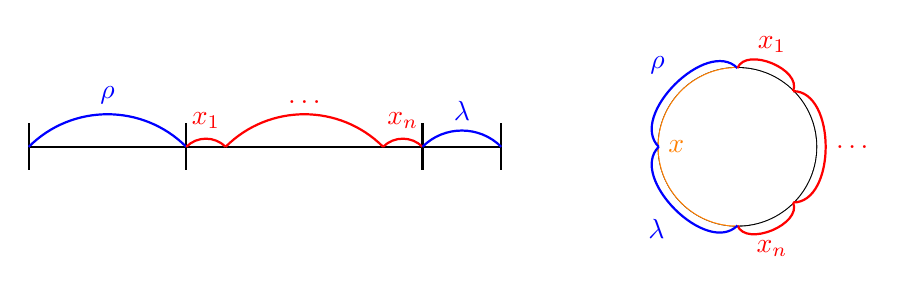
\begin{tikzpicture}
    \def \r {1}
    \coordinate (A) at (-9,0);
    \coordinate (B) at (-7,0);
    \coordinate (C) at (-4,0);
    \coordinate (D) at (-3,0);

    \draw[thick] (A) -- (D);
    \draw[thick] (A) -- ++(0,-0.3);
    \draw[thick] (A) -- ++(0,0.3);
    \draw[thick] (B) -- ++(0,-0.3);
    \draw[thick] (B) -- ++(0,0.3);
    \draw[thick] (C) -- ++(0,-0.3);
    \draw[thick] (C) -- ++(0,0.3);
    \draw[thick] (D) -- ++(0,-0.3);
    \draw[thick] (D) -- ++(0,0.3);

    \draw[thick,blue, bend left = 45] (A) to node[midway, above, blue]{\(\rho\)} (B);
    \draw[thick,red, bend left = 45] (B) to node[midway, above, red]{\(x_1\)} (-6.5,0);
    \draw[thick,red, bend left = 45] (-6.5,0) to node[midway, above, red]{\(\ldots\)} (-4.5,0);
    \draw[thick,red, bend left = 45] (-4.5,0) to node[midway, above, red]{\(x_n\)} (C);
    \draw[thick,blue, bend left = 45] (C) to node[midway, above, blue]{\(\lambda\)} (D);
    

    \draw[thick] (0,0) circle (\r);
    \draw[thick,orange] (0,-\r) arc[start angle=270, end angle=90, radius=\r] -- cycle;
    \fill[white] (0,0) circle (\r);
    \node[anchor=west, orange] at (-\r,0) {\(x\)};
    \draw[thick,blue, bend left = 90] (-\r,0) to node[midway, above left, blue]{\(\rho\)} (0,\r);
    \draw[thick,red, bend left = 90] (0,\r) to node[midway, above, red]{\(x_1\)} ({cos(45)},{sin(45)});
    \draw[thick,red, bend left = 90] ({cos(45)},{sin(45)}) to node[midway, right, red]{\(\ldots\)}({cos(-45)},{sin(-45)});
    \draw[thick,red, bend left = 90] ({cos(-45)},{sin(-45)}) to node[midway, below, red]{\(x_n\)} (0,-\r);
    \draw[thick,blue, bend left = 90] (0,-\r) to node[midway, below left, blue]{\(\lambda\)} (-\r,0);
    
  \end{tikzpicture}
  \caption{Rappresentazione grafica della definizione di codice circolare}
\end{figure}

\begin{example}{}
  Il codice \(X = \set{ab,ba,bb}\) non è circolare. Considerando infatti la parola \(abab\). Si ha che, fissando \(\rho = a, \lambda = b\) che \(\lambda\rho = ba \in X\) e che \(\rho ba \lambda = abab \in \set{\rho}X^*\set{\lambda}\).
  Passando alla fattorizzazione circolare, è possibile ottenere \(abab\) nei seguenti modi:
  \begin{figure}[H]
    \centering
    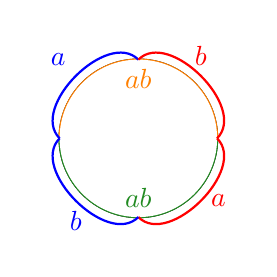
\begin{tikzpicture}
      \def \r {1}
      \draw[thick] (0,0) circle (\r);
      \draw[thick,orange] (-\r,0) arc[start angle=180, end angle=0, radius=\r] -- cycle;
      \draw[thick,ForestGreen] (-\r,0) arc[start angle=180, end angle=360, radius=\r] -- cycle;
      \fill[white] (0,0) circle (\r);
      \node[anchor=north, orange] at (0,\r) {\(ab\)};
      \node[anchor=south, ForestGreen] at (0,-\r) {\(ab\)};
      \draw[thick,blue, bend left = 90] (-\r,0) to node[midway, above left, blue]{\(a\)} (0,\r);
      \draw[thick,red, bend left = 90] (0,\r) to node[midway, above, red]{\(b\)} (\r,0);
      \draw[thick,red, bend left = 90] (\r,0) to node[midway, right, red]{\(a\)}(0,-\r);
      \draw[thick,blue, bend left = 90] (0,-\r) to node[midway, below, blue]{\(b\)} (-\r,0);
    
    \end{tikzpicture}
    \hspace{2cm}
    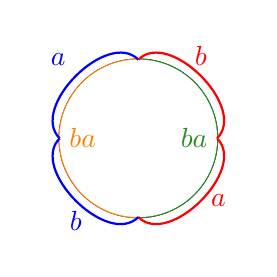
\begin{tikzpicture}
      \def \r {1}
      \draw[thick] (0,0) circle (\r);
      \draw[thick,orange] (0,-\r) arc[start angle=270, end angle=90, radius=\r] -- cycle;
      \draw[thick,ForestGreen] (0,-\r) arc[start angle=-90, end angle=90, radius=\r] -- cycle;
      \fill[white] (0,0) circle (\r);
      \node[anchor=west, orange] at (-\r, 0) {\(ba\)};
      \node[anchor=east, ForestGreen] at (\r,0) {\(ba\)};
      \draw[thick,blue, bend left = 90] (-\r,0) to node[midway, above left, blue]{\(a\)} (0,\r);
      \draw[thick,red, bend left = 90] (0,\r) to node[midway, above, red]{\(b\)} (\r,0);
      \draw[thick,red, bend left = 90] (\r,0) to node[midway, right, red]{\(a\)}(0,-\r);
      \draw[thick,blue, bend left = 90] (0,-\r) to node[midway, below, blue]{\(b\)} (-\r,0);
    
    \end{tikzpicture}
    \caption{Rappresentazione grafica di due fattorizzazioni circolari per la parola $abab \in X^{*}$.}\label{fig:circular_factorization}
  \end{figure}
  Inoltre, qualsiasi codice che contenga una parola che è potenza di una lettera non può essere circolare.
  Questo si può banalmente vedere considerando il caso in cui \(a^n \in X\) con \(a \in A\). Si ha necessariamente che \(a^{2n} = a^{\frac{n}{2}} a^n a^{\frac{n}{2}} \in X^*\) e dunque la fattorizzazione non è circolarmente univoca.
\end{example}

\begin{proposition}{Chi troppo vuole...}
  Sia \(X\) codice su \(A\) finito, circolare e massimale. Allora \(X = A\).
\end{proposition}

\begin{proof}
  Per \Cref{cor:schutz_maximality_completeness} e dalla \Cref{prop:finite_complete_codes_contains_powers}, sappiamo che se \(X\) è massimale e finito, \(\forall a \in A, \exists n_a \geq 1 \st a^{n_a} \in X\).
  Poiché \(X\) è circolare, \(\forall a, n_a = 1\).
  Dunque \(A \subseteq X \implies X = A\) e $A$ è codice massimale su \(A^*\).
\end{proof}

\begin{theorem}{Restivo}
  Sia \(X\) codice su \(A\). Allora
  \begin{enumerate}
    \item \(X\) codice a ritardo di sincronizzazione finito \(\implies X\) circolare e a \keyword{parassitismo limitato}.
    \item \(X\) codice regolare, circolare e a parassitismo limitato \(\implies X\) codice a ritardo di sincronizzazione finito
  \end{enumerate}
\end{theorem}

\begin{note}{}
  Il parassitismo (limitato) non è stato trattato nel corso, poiché esula dagli argomenti principali.
  In maniera informale, un codice \(X\) ha parassitismo se esistono parole di \(X\) che contengono al loro interno parole di \(X^*\)
  Si parla di parassitismo limitato se esiste un limite superiore \(p\) alla lunghezza delle parole di \(X^*\) che possono essere contenute all'interno di parole di \(X\).
  Più formalmente,
  \[X \text{ ha parassitismo} \iff (A^+X^* A^*\cup A^*X^*A^+) \cap X \neq \emptyset\]
  \[X \text{ ha parassitismo limitato} \iff \exists p > 1 \st A^*X^p A^* \cap X = \emptyset\]

  Ciò che è d'interesse per questo corso, è che qualsiasi codice finito ha necessariamente parassitismo limitato.
\end{note}

\begin{corollary}{}
  Sia \(X\) codice finito, allora \(X\) codice a ritardo di sincronizzazione finito \(\iff X\) circolare.
\end{corollary}

\begin{corollary}{}
  Un codice a ritardo di sincronizzazione finito, binario e adattato a una sorgente propria \textbf{non} è ottimale (a meno che \(\# \SCal = 2\)).
\end{corollary}

\begin{proof}
  Dal corollario precedente, un codice a ritardo di sincronizzazione finito e adattato a una sorgente propria è circolare.
  Sappiamo inoltre che un codice binario ottimale è anche massimale.
  Dunque, per la proposizione precedente, l'unico codice finito binario circolare ottimale è l'alfabeto stesso, che però non è adattato a una sorgente propria con più di due simboli.
\end{proof}

Dunque, abbiamo finora scoperto che un codice finito ha ritardo di sincronizzazione finito se e solo se è circolare. Tuttavia, la verifica manuale della circolarità di un codice può essere ardua. Per fortuna, esiste un metodo iterativo di facile applicazione.

\begin{definition}{Insiemi resto modificati}
  Sia \(X\) codice su \(A\). Definiamo l'insieme dei \keyword{resti modificati} di \(X\) come
  \begin{equation*}
    R_n'(X) = \begin{cases}
    Suff(X)\setminus (X \cup \set{\varepsilon}) & n = 1\\
    {R_{n-1}'(X)}^{-1}X \cup X^{-1}R_{n-1}'(X) & n > 1
    \end{cases}
  \end{equation*}
\end{definition}

\begin{theorem}{Levenshtein}
  \(X\) circolare \(\iff \exists n \geq 1 \st R_n'(X) = \emptyset\)
\end{theorem}

\begin{observation}{}
  Per \(X\) codice (finito),
  \[R_1 = X^{-1}X\setminus \set{\varepsilon} \subseteq Suff(X) \setminus (X \cup \set{\varepsilon}) = R_1' \implies \forall n \geq 1, R_n \subseteq R_n'\]
  Questo è un altro modo per dimostrare che se \(X\) ha ritardo di sincronizzazione finito, allora ha ritardo di decodifica finito.
  Infatti se ha ritardo di sincronizzazione finito, allora ha \(R_n' = \emptyset\) per qualche \(n\), dunque anche \(R_n = \emptyset\) per lo stesso \(n\), e quindi ha ritardo di decodifica finito per teoremi visti prima.
\end{observation}

\begin{example}{}
  \(X = \set{a,ba,bb}\) \textbf{non} è circolare.
  Infatti \(R_1' = Suff(X) \setminus (X \cup \set{\varepsilon}) = \set{b}\).
  Inoltre, \(R_2' = {R_1'}^{-1}X \cup X^{-1}R_1' = \set{a,b}\).
  \(R_3' = \set{\varepsilon, a ,b}\),\(R_4' = \set{\varepsilon, a ,b, ba,bb} = R_n' \forall n \geq 4\).

  Invece, \(X' = \set{ab,aab}\) è circolare: \(R_1' = \set{b}, R'_2 = \emptyset\).
  
  Anche \(X'' = \set{ab,aba,ba^3,b^2a}\) è circolare:
  \(R_1' = \set{a,b,a^2,ba,a^3}, R_2' = \set{b,ba,a^3,a^2}, R_3' = \set{a^3,ba,a^3}, R_4' = \set{a^3}, R_5' = \emptyset\)
\end{example}

